% \chapter{Building Energy Model of DCs}
% \label{chp:bem}

% For the conference, need \citepp{}, otherwise for dissertation replace with \citep{}

\section*{Abstract}	% Section headings need to be upper and lower case.
% -------------------------------------------------------------------------------------------------------------------------------

\addtocounter{section}{1}

% Relate to title
% Towards Energy Simulations for Proportionally Designed and Controlled Data Centers

Expressing site-specific load profiles and hardware specifications that reflect the information technology (IT) processes inside data centers have always been a challenge to do either benchmarks of building energy performance or predictive controls. As a substitute, data center building models usually assume naive hour-day-week schedules that don't align simulated operations with the weather profiles. 
This paper demonstrates a method towards using more representative load profiles in data center energy models by deriving the profiles based on global usage patterns of an internet platform. It is the first attempt to illustrate the coupling of an external signal with EnergyPlus as an indicator of IT load in a data center. 

% -------------------------------------------------------------------------------------------------------------------------------
\section{Introduction}
% -------------------------------------------------------------------------------------------------------------------------------

\added{This paper describes a data center (DC) building energy simulation framework. The framework is based on EnergyPlus as the physical model of the building operations and an externally implemented network traffic schedule as an indicator of the IT load. Namely, the target applications for these frameworks are the hyper-scale facilities that house global services such as social networks and search engines. For this class of facilities, the significance of network traffic to DC operations is exemplified by the sudden change in peoples internet usage behaviors due to the COVID-19 pandemic. Through the pandemic, DCs across the globe have seen a disruptive shift in user traffic patterns that were not known just weeks prior to the first stay-in-place orders. Given this timely example, it is imperative that DC operators be able to simulate their facilities to verify that their infrastructure can handle these types of shifts in traffic. However, presently there is a lack of publicly available information about how to build such simulations. 


The contribution of this work is two-fold. First, it provides a demonstration for characterizing data centers and IT equipment in EnergyPlus. Second, by deriving the workload profile from network traffic, this work provides a perspective for reasoning about temporal profiles of the workloads that hyper-scale data centers must support.}

\deleted{DCs are the backbone of today's internet based economy. From an energy perspective, in the U.S DCs consume around 2\% of the total energy produced, with 10 times or more power density then conventional office buildings. Through the COVID-19 pandemic, DCs across the globe have seen a disruptive shift in traffic and workload patterns. Given this timely example, it is warranted that DC operators be able to simulate their facilities to verify that their infrastructure can handle these types of shifts in traffic. This research proposes that dynamic computational workloads of DCs can be sufficiently and accurately characterized with current building energy modeling tools to allow such simulations.

The methodology presented in this article couples a network model indicative of internet traffic with the building power load profiles. The effectiveness of such a model is demonstrated by extending the model to five DCs dispersed globally and comparing their results. The framework can be used by architects and designers to assess building energy models of DCs and to provide an indicator of opportunistic thermal headroom during non-design day conditions.}

\deleted{In 2020 U.S DCs are projected to consume 73 billion kWh \citep{Shehabi16}. This value is significantly curtailed from the trends documented in a 2007 Report to Congress \citep{koomey07}. The report provided evidence of unsustainable energy demands by DCs as the industry expanded, based-on the industry's growth observed from the early 2000’s. Koomey's report was a medium that spread awareness of the problem. Since then various opportunities for energy reduction have been identified and implemented by IT equipment and facility systems architects.

Two specific engineering choices have had profound benefits towards DC energy efficiency. First, proportional power and thermal control of DC components is now enabled across all dimensional scales. An example of a millimeter scale proportional control is of central processing units (CPU) with dynamic frequency voltage scaling (DFVS) \citep{osullivan15}, \citep{barroso18}, \citep{joshi12}.

To appreciate the DFVS’ correlation across the distinct technical domains of computer systems and buildings it should be noted that legacy hardware operations did not proportionally utilize power or cooling with their IT workloads. Most intuitively, this meant that an IT device consumed nearly the same amount of power whether it was idle or being 100\% utilized. The latest generation of IT equipment have much better proportional control enabled by variable fan speeds, variable power draw, and variable heat dissipation resulting from workload dependent power draw enabled with DFVS.  

Second, power and thermal constraints have been relaxed compared to legacy practices. As an example, led by hyper-scale early adopters like Facebook,dual conversion power typologies are now being replaced with bypass systems \citep{Park15}. The removal of dual conversion power systems not only saves capital costs associated with complex uninterruptible power distributions, but it also saves operational expense by requiring power rectification at the IT point of connection only. 

Omission of dual conversion power distribution systems is one example that has been enabled by deep integration across IT and building systems power architectures. Another example is the collaboration between thermal architects of IT and buildings that led to the expansion of the operational environment's thermal psychometric window for IT equipment. An expanded psychrometric window increases the opportunity to exploit free cooling modes across various climate zones \citep{ASHRAETC9.9}. In more aggressive implementations, some DC operators have gone beyond the opportunistic use phase power usage effectiveness optimality and have discarded compressor-based equipment from their cooling plants completely. Compressor-less cooling plants offer significant capital costs savings as-well as the operational energy and maintenance costs \citep{Mulay18}.} 

\added{DCs have 10 times the power density of conventional buildings. With this density, it is essential that during the design phase designers have access to representative building energy models to size equipment and to validate jurisdictional compliance. However, these building energy models are typically put on the shelf once the facility is turned over to the operational teams. With much of the life cycle costs of a data center attributed to the use-phase, having building energy models that represent the cyber-physical dynamics of their facility can be valuable to support operational decisions too.

In this work, wide area network traffic bandwidth is demonstrated as a proxy for IT loads in data center buildings. However, any technique that characterizes a fine grain coupling between the IT workloads and the building systems would be valuable for hyper-scale DCs running online platforms such as social media sites, search engines, or public cloud services. These platforms are typically distributed through out the world for redundancy and performance objectives for their global user base. In terms of building scale, each data center can scale beyond a hundred thousand square meters with 100s of MW of power. Even with the ever growing needs for hyper-scale data centers today, there is a lack of publicly available literature which discuss coupling building energy models with IT operations to help operators reason about actual service workloads and their building's performance} 

In the recent past, the power usage effectiveness metric ($PUE$) as defined by Equation~\ref{eq:pue} has been a key performance indicator for DC facilities architects and facilities operators. 

    \begin{equation} \label{eq:pue}
    PUE=\frac{E_{total}}{E_{IT}} 
    \end{equation}
    \begin{center}
    $E_{total}$ = Total Power Used at Facility
    
    $E_{IT}$ = Power Consumed by IT Equipment
    \end{center}
    \vspace{.2cm}
    


% \deleted{\begin{equation}\label{eq:pue}
%   PUE  = \frac{Total\; Power\; Used\; at\; Facility}{Power\; Consumed\; by\; IT\; Equipment}
% \end{equation}}

\deleted{In operations} \added{The $PUE$ is a intuitive metric to reason about. In consideration of the $PUE$, the mechanical inefficiencies and electrical distribution losses external to the IT equipment contribute to the difference between the numerator and denominator of Equation~\ref{eq:pue}}. In operations, the facilities and IT parameters change simultaneously together in a continuous sequence, lending to accurate real time evaluations. However, the continuous states of IT workloads and ambient environmental conditions makes design time PUE calculations complicated. The complications drive DC building designers to evaluate the efficiency metric, \deleted{at}\added{by averaging} discrete step-wise \added{(hour-day-week) workload values and taking the worst case values to benchmark the facility}.

\deleted{Like the PUE calculations, DC building energy models are also reasoned about through these coarse step loads. The step-wise inputs are sufficient for two things. First, for sizing equipment which must support the nominal DC capacity in any possible operational condition with the bounds of the basis of design. Second for producing energy models which are suitable for prescriptive compliance reviews; allowing  municipalities to normalize across different DCs in their jurisdiction.} 

However, without accounting for continuous workload profiles these coarse models misrepresent the part-load operations of the DC and inaccurately quantify total energy demands over a time period. The misrepresentation has significant impacts throughout the life of the hardware deployed in these DC facilities. For example without realistic coincident alignment of workloads and ambient conditions, the thermo-electric equipment whose energy use is dependent on workloads and ambient temperatures may be over-sized for significant portions of their operational times. \added{Yet, during these times the equipment are still allocated their nameplate power draws regardless of their lower operational points. The allocation translates to power being reserved regardless of real demand}. 

The simulations demonstrated in this research allow for more realistic evaluations of DC energy use. These more realistic evaluations are useful for two things. First, operators can use the realistic cyber-phsyical models to simulate the DC building performance under perceived usage changes. Second, by exposing the facility's power and cooling equipment headroom for non-design day conditions they can enable DC operators to opportunistically oversubscribe the IT loads. Such a oversubscribing scheme can be implemented by extending the electrical over-subscription \added{leading to free capacity} schemes presented by Li \citep{Li18} \added{when coupled with predicative modeling techniques}.

The contribution of this work is the \added{demonstration of} an IT load aware building energy model that integrates \added{an external Python script to dynamically reset the IT load that must be cooled within} \deleted{a dynamic time-series of IT power with} EnergyPlus. \deleted{This method can further be expanded by exploiting the real-time headroom at coincident IT load and environmental conditions vs. the design-day capacities of the facilities equipment for opportunistically increasing the supportable IT workloads that are constrained by power, leading to free capacity.} The rest of the paper discusses specific modules that one of the authors built to couple the building systems and IT. 

In the next section, similar works on data center energy models are discussed. In the subsequent section, Methodology, the methods and reasoning behind the modules developed in this work are discussed. The results from implementing these methods are then presented in the Results section followed by a Discussion section in which the authors reason about the article's results and claims. The paper then concludes by highlighting the contribution and identifying opportunities for extending this work. 

\deleted{As an example of free capacity, consider a design day dry-bulb temperature of \deleted{110$^{\circ}$F}\added{105$^{\circ}$F}. When a peak in IT workload occurs on a more favorable day, say 95$^{\circ}$F, the computer room air conditioner heat rejection equipment needs less than 50\% of the designed power value \citep{liebert20}. With a slight modification in the electrical infrastructure, this difference can opportunistically be allocated to IT workloads. However slight the the electrical modification, the decision is most cost effectively made during the design phase of the the facility.}

\deleted{This article first provides a background for the need of IT coupled DC building energy models and discusses similar works. Then a novel simulation methodology is proposed for extending the existing DC modeling capabilities of EnergyPlus to allow for dynamic IT workload profiles in it. Using the proposed method, two simulations are performed and their comparisons are discussed. The first of the two models serves as a baseline, where the peak IT load is constant throughout the year. In the second simulation, a dynamic IT workload is expressed. A comparison of the results are then presented in the Results from Proposed Method section. The article concludes with a summary of the work and outlines future research that leans on this model.}

% -------------------------------------------------------------------------------------------------------------------------------
\deleted{\section{Background}}
% -------------------------------------------------------------------------------------------------------------------------------

\deleted{Over the last 15 years, the deployment paradigm of DCs has transformed from monolithic deployments of high-end devices to heterogeneous deployments of cost-efficient commodity equipment that dwarf the their predecessor in all dimensional scales. With an appropriate title, in Warehouse Scale Computer Barroso et al. describe their DC design and operational experiences in this new paradigm \citep{barroso18}. The work provides details from the software platforms to the industrial sized power and cooling plants found at mega-Watt scale DC campuses. This work provides compelling financial incentives for designs and operations that prioritize proportional energy use at these massive scales. Furthermore, Barroso provides explicit workload profiles from real DCs that lend themselves to opportunistically oversubscribe the capacity of the mechanical and electrical infrastructure in proportion to the IT workloads.

It is evident by the preceding discussions that energy efficiency of DCs is dependent on the proportional power management across all components found in them. However, the PUE metric presented above does not capture the end to end electro-mechanical efficiency of DCs as it misses the IT inefficiencies. For IT devices, several methods for enhancing the proportional power management have been summarized by O'Sullivan \citep{osullivan15}. O'Sullivan presents design solutions for those methods and demonstrates that through workload proportional computing, it is technically feasible to optimize the end to end electro-mechanical efficiency of the hardware. The control feedback loops that O'Sullivan describes also lend themselves to be leveraged by building systems. As an example, return air temperature readings at air handlers can be supplemented with input power demand values to more effectively control air handling fan speeds and their cooling stages. 

Awareness of the total power demands jointly by the building system's and the IT telemetry leads to another area of integration, power capping. Power capping throttles the CPU power cycles, similar to load shedding schemes implemented by power utility companies for consumer energy use. A novel power capping strategy is proposed by Li \citep{Li18}. Li's power capping methods provide a means for building systems to actively exploit the device level power management capabilities of Intel’s CPU Node Manager feature (\citep{intel15}. Intel's CPU Node Manager enables the DC infrastructure telemetry to observe building telemetry (ie from power meters on rack power strips) and throttle the CPU when the workloads demands encroach the facilities power, risking an upstream circuit-breaker trip.

Given the various operational interdependence between building and IT systems, traditional building energy modeling techniques have failed to suffice for DCs \citep{Beatty15}. Beatty's critique resonates with the three influential DC energy evaluation methods. Those methods either are directly enforced or adopted through reference by authorities having jurisdiction across the US. 

The first and most influential method is ASHRAE 90.4, the Energy Standard for DCs (ASHRAE, 2019). Compliance with the standard can be achieved through prescriptive or performance-based methods. EnergyPlus simulations are one of the approved methods for performance-based compliance along with spreadsheet-based methods. Regardless of the method, the standard allows various subsystems to be isolated for compliance based on whether they are mechanical or electrical load components (MLC/ELC) which fall back on prescriptively defined threshold values.

The second influential method is a part of the certification process for the US Green Building Council's LEED program. LEED requires prescriptively defined performance calculations to validate compliance \citep{LEED16}. Compliance with the LEED method is done through a spreadsheet tool, where designers input their DC IT characteristics along with the properties of the IT power distribution system. The strict prescriptive boundary set by LEED accounts for the electro-mechanical efficiency at discrete design points of specific devices but does not account for the computational workloads. The computational workloads are known to significantly influence IT equipment power draw \citep{marculescu20}.  

The third method, adopted by many power utility companies for compliance with their rebate program comes from the Pacific Gas and Electric Company (PGE). PGE method mandates an documented IT load profile to indicate the part load conditions, where the profile is established with 1-month of trend data for new construction. In industrial practice however, it takes several years to fully populate a DC with equipment and DC workloads, like the weather, have seasonal periods of cyclic behavior \citep{zhuang15}.}

% -------------------------------------------------------------------------------------------------------------------------------
\section{Similar Works}
% -------------------------------------------------------------------------------------------------------------------------------

As described above, PUE is not the comprehensive metric for DC energy efficiency. By acknowledging that PUE does not account for IT equipment efficiency, Perolini provides a coordinated control strategy across IT workload and building infrastructure based on network queuing theory \citep{parolini12}. Perolini logically composes a set of IT systems and supporting infrastructure as a singular cyber physical system network graph. Hierarchically structured quality of service (QoS) values is common among Perolini and Li, who uses the QoS to optimize IT performance in terms of the power distribution system \citep{Li18}. Both authors dynamically tune IT with the facilities infrastructure systems. In terms of exploiting the QoS,  the fundamental difference between these two works is that Li considers the IT workload as the controlled variable bound by the facility's power distribution systems and Perolini considers the cooling equipment as the controlled variable bound by the IT workload. In their recognition of lower QoS DC workloads as being preemption tolerant and higher QoS as time sensitive workloads; these methods allow over-subscription of power and thermal capacities without any service level performance degradation. 

DC cooling systems have been algorithmically coupled with DC IT workloads by Wei in \citep{wei17}. They use a reinforcement learning agent that is aware of the DC's thermal state in real-time. The agent acts as a controller of the HVAC equipment and respective IT traffic balancer, where the balancer migrates work between two or more DCs. In the work they demonstrated that when given a state-action pair and an objective function, the agent takes a control action in a given state to reduce power while allowing the IT system to meet it's performance objective in terms of processing latency. The state-action pairs are optimized with an objective function that values the power demand along with a IT performance metric at a given time-step. Wei's work was limited to DCs located in mixed use buildings, where the cooling system had some fungibility with other parts of the building, allowing waste energy from the DC to be reclaimed to heat the other parts. Nonetheless, their work is similar to this research in that it also integrated EnergyPlus together with Python.

% -------------------------------------------------------------------------------------------------------------------------------
\section{Methodology}
% -------------------------------------------------------------------------------------------------------------------------------

In this section a dynamic workload-profile based energy simulator is introduced and the simulation is described in detail. First, an overview of this work's cross platform software integration is presented. Then details about each of the two main components, namely EnergyPlus and Python based traffic models, are discussed.  As shown in Figure~\ref{img_ep_py}, the proposed simulator uses Python to reset the DC IT load for each time-step. In the subsequent modeling time-step, the EnergyPlus models run with the externally revised variables. The basic process loop of the simulator is illustrated in Figure~\ref{fig:dyna-bem}.

\begin{figure} [!h]
\centering
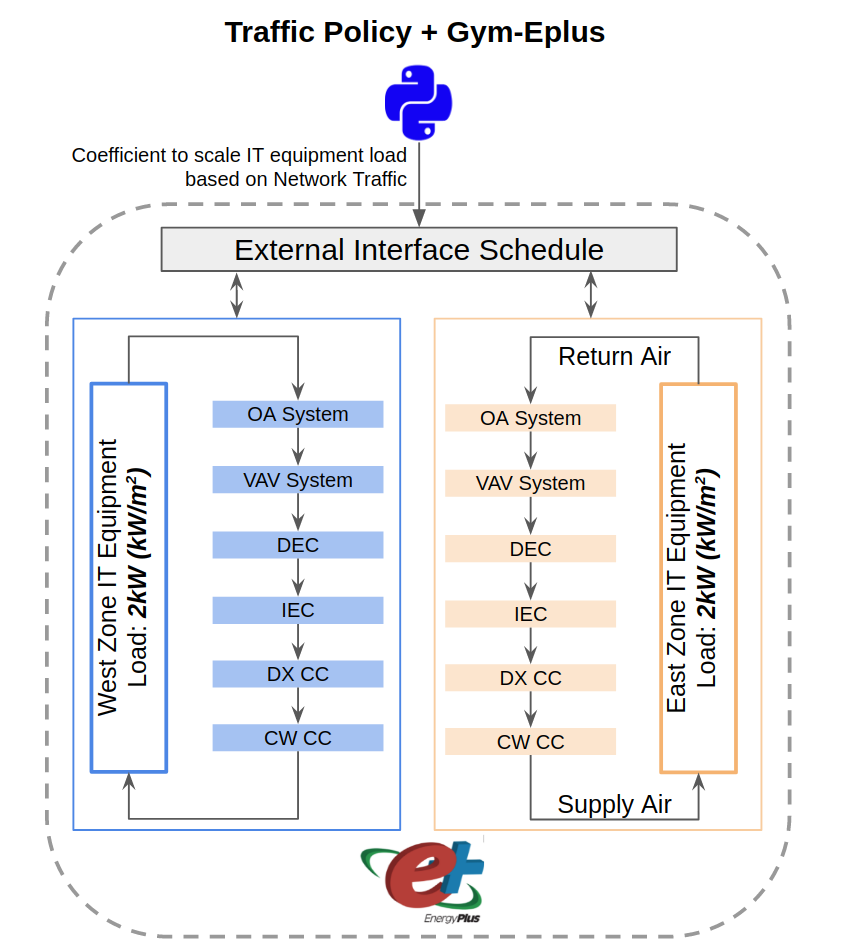
\includegraphics[scale=.25]{building_energy_model/TowardsEstimatingtheEcologicalCostsofInternetServices/paper_latex/img/python_eplus.png}
\caption[EnergyPlus and Traffic Model.]{EnergyPlus and Traffic Model.}
\label{img_ep_py}
\end{figure}

\begin{figure}
\centering

\includegraphics[scale=.10]{traffic_profile/images/agent_bem.png}
\caption{Dynamic Process Flow between EnergyPlus and the Python Agent.}
\label{fig:dyna-bem}
\end{figure} 

The simulator \deleted{allows}\added{integrates} algorithms that are aware of network traffic profiles programmed in Python \deleted{to interact} with EnergyPlus through the Building Controls Virtual Test Bed (BCVTB) \citep{wetter16}. The BCVTB interface from Gym-EPlus \citep{zhang19} is used to implement the interaction. \deleted{Python is chosen for the interface function due to its flexibility and the the granular level of program control and EnergyPlus is chosen due to it's established efficacy with building modeling. EnergyPlus is the US Department of Energy's state-of-the-art building modeling software. It features an extensible physics-based building thermodynamic and psychrometric modeling engine to simulate sub-hourly energy demands and occupant comfort values.} \added{This work extends Gym-Eplus capability by making it reset the IT load in DCs in addition to its thermal reset features. DCs have been explicitly supported in EnergyPlus since Version 8.3.0. Using the already supported DC variable for CPU load schedules in EnergyPlus, the xml file configuration as shown in Figure~\ref{cfg_xml} couples the Python module with EnergyPlus.}

\begin{figure} [!h]
 \lstset{
    language=xml,
    tabsize=3,
    %frame=lines,
    % caption=Test,
    label=cfg_xml,
    frame=single,
    rulesepcolor=\color{gray},
    xleftmargin=20pt,
    framexleftmargin=15pt,
    keywordstyle=\color{blue}\bf,
    commentstyle=\color{OliveGreen},
    stringstyle=\color{red},
    numbers=left,
    numberstyle=\tiny,
    numbersep=5pt,
    breaklines=true,
    showstringspaces=false,
    basicstyle=\tiny,
    emph={food,name,price},emphstyle={\color{magenta}}}
    \lstinputlisting{building_energy_model/code_cfg.xml}
\caption[EnergyPlus Variables reset by Python.]{EnergyPlus variables.cfg used to integrate Python and EnergyPlus. Other variable maps from GymEplus are listed in the variable.cfg, but not used in these simulations.}
\label{cfg_xml}
\end{figure}


\added{The baseline EnergyPlus model of the data center is adapted from Moriyama \citep{moriyama18}. Moriyama's building shell consists of two data center rooms. The first room, the West Zone is 232 square meters and the second room, East Zone, is 259 square meters. Each data center room has dedicated mechanical and electrical equipment that are symmetrical to each other. Throughout the simulations the building envelope, mechanical, and electrical modeling objects are not modified from the baseline. However, for this research, as the goal is to represent hyper-scale DCs; the IT equipment objects are changed to closer resemble the current practices in this class of DCs based on one of the author's industrial experience.}

% To closer resemble the current practices, the EnergyPlus IT object is defined based on one of the author's experience leading DC projects for severel large search engines and social media companies.   

\added{Three statically configured changes are made to the baseline model's ITE object. Namely the changes include the values for server inlet temperature, fan power ratio compared relative to the overall server power, and the CPU power density fields are changed. The typical EnergyPlus ITE object for each zone is provided in Figure~\ref{ite_object}. First on line 16, the server entering air temperature is changed to $25^{\circ}C$ from $15^{\circ}C$. Second, on line 12 the fan power fraction is changed to 0.10 from 0.40. The last static variable change increases the load density of the data center to 2 $\frac{kW/m^2}$ from 0.2 $\frac{kW/m^2}$ on line 8. Details on how this power density was derived is provided later in Algorithm~\ref{rack_power_counts}}.


\begin{figure} [!h]
 \lstset{
    language=fortran,
    tabsize=3,
    %frame=lines,
    % caption=Test,
    label=cpu_load_schedule_reset,
    frame=single,
    rulesepcolor=\color{gray},
    xleftmargin=20pt,
    framexleftmargin=15pt,
    keywordstyle=\color{blue}\bf,
    commentstyle=\color{OliveGreen},
    stringstyle=\color{red},
    numbers=left,
    numberstyle=\tiny,
    numbersep=5pt,
    breaklines=true,
    showstringspaces=false,
    basicstyle=\tiny,
    emph={food,name,price},emphstyle={\color{magenta}}}
    \lstinputlisting{building_energy_model/code_ITE.idf}
\caption[EnergyPlus IDF ITE Object]{EnergyPlus ITE Object Defintion. New features of EnergyPlus 8.9 are denoted with *.}
\label{ite_object}
\end{figure}

\added{The only dynamic variable change to the ITE object definition specifies the dynamic CPU Loading Schedule\_RL on line 10 of Figure~\ref{ite_object}. This new schedule replaces the original schedule, CPU Loading Schedule. Both of these schedules are shown in the IDF snippet in Figure~\ref{cpu_load_reset}. The CPU Loading Schedule\_RL is called from the IDF as an external interface through the BCVTB. For the BCVTB and EnergyPlus interface, this new schedule is mapped between the two software platforms in the variable.cfg file on line 38. Then at each time-step, a value for the CPU load is passed from Python to EnergyPlus. The passed value is multiplied by the CPU power density from line 8 of Figure~\ref{ite_object} for the simulation time-step.} 

\begin{figure} [!h]
 \lstset{
    language=fortran,
    tabsize=3,
    %frame=lines,
    % caption=Test,
    label=cpu_load_schedule_reset,
    frame=single,
    rulesepcolor=\color{gray},
    xleftmargin=20pt,
    framexleftmargin=15pt,
    keywordstyle=\color{blue}\bf,
    commentstyle=\color{OliveGreen},
    stringstyle=\color{red},
    numbers=left,
    numberstyle=\tiny,
    numbersep=5pt,
    breaklines=true,
    showstringspaces=false,
    basicstyle=\tiny,
    emph={food,name,price},emphstyle={\color{magenta}}}
\lstinputlisting{building_energy_model/code_cpu_load_schedule.idf}
    
% \lstinputlisting[language=fortran]{code_cpu_load_schedule.idf}
\caption[EnergyPlus IDF load Reset]{EnergyPlus IT load reset schedule definitions. The Schedule: Compact is replaced with the schedule defined in the External Interface: Schedule.}
\label{cpu_load_reset}
\end{figure}

\added{There are two ways to input the IT power load into EnergyPlus. The first is the unit count and unit-power method. The second is the power-density method. As seen above the floor area density method is used for this work. The density method is more conducive to scaling with the building size than the unit-power method. Algorithm~\ref{rack_power_counts} indicates the steps used to translate the properties from an actual hyper-scale data center to Moriyama's model. The density ($\rho$) is simply the product of the total provisions power for the IT equipment on the server floor ($P_f$) and the total server floor area ($A_F$).}

\added{Although expressing the IT density as a constant value over the entire floor area suffices for EnergyPlus' view of the IT load as a lumped thermal parameter, it is a naive representation of the power distribution on the floor. In reality racks are not placed evenly across the entire server floor, but are placed in rectilinear arrangements, as represented by $A_r$ in Algorithm~\ref{rack_power_counts_bem} and illustrated in \ref{img_server_room_bem}. By following the equations in Algorithm~\ref{eq:area_for_racks}, the rack counts and rack unit densities can be obtained and the method of entry can be changed.}

\begin{figure} [!h]
\centering
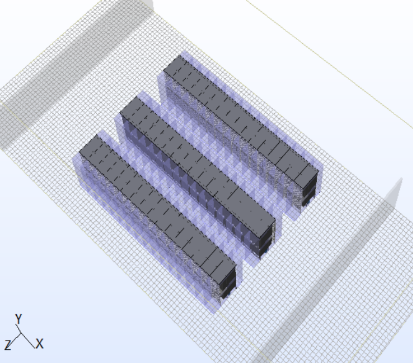
\includegraphics[scale=.5]{methodology/images/server_room.png}

\caption[Server room layout]{Server room layout. The gray elements in the figure are the hot aisles and the light purple elements are the server racks. The objective of the cited work was to determine the optimal spacing of adjacent racks across hot-aisles.  Image from \cite{sahini16}}
\label{img_server_room_bem}
\end{figure}
  \begin{algorithm}
    \caption{Rack Counts from Building and Power Properties}
    \begin{algorithmic}

      \STATE $\rho= \frac{P_{f}}{A_{F}}$

      \STATE $A_{r}= A_{f} \times F_{f}$
      \STATE $R_{\#}= \frac{A_{r}}{R_{a}}$
      \STATE $P_{rs} = \frac{P_f \times (1-F_{n})}{R_{\#}}$
      \STATE $P_{rn} = P_{rs} \times F_{n}$
      \STATE $P_r = P_{rs} + P_{rn}$
      
      \STATE{\bf{Where}}: \\
        \hspace{.2in}$\rho$ = Power Density of server floor. This value is used in the EnergyPlus Models. \\
        \hspace{.2in}$A_{f}$ = Total floor area.  \\
        \hspace{.2in}$A_{r}$ = Area available for rack deployment.  \\
        \hspace{.2in}$R_{a}$ = Rack footprint area. \\
        \hspace{.2in}$R_{\#}$ = Rack count.\\
        \hspace{.2in}$P_{f}$ = Provisioned power for IT for server floor.\\
        \hspace{.2in}$P_{rs}$ = Power for rack server equipment. \\
        \hspace{.2in}$P_{rn}$ = Power for rack network equipment. \\
        \hspace{.2in}$P_{r}$ = Total power of rack. \\
        \hspace{.2in}$F_{f}$ = Fraction of $A_{f}$ that is deployable with Racks.\\
        \hspace{.2in}$F_{n}$ = Fraction of power to rack allocated to network devices.
        
    \end{algorithmic}
    \label{rack_power_counts_bem}
  \end{algorithm}

\deleted{Without the Python feedback loop, EnergyPlus is a hermetic suite in which simulation run-parameters are defined in a configuration file; namely the IDF. In the default case, EnergyPlus modeling workflow serially runs the simulations \deleted{and then users get to review the results of each simulation at} \added{to} completion. Iterating on the parametric values requires \added{manual} editing of the IDF file and re-running of the entire simulation. This proposed simulation specifically defines a loop in Python which iterates over a list of load coefficients derived from the network traffic corresponding to the cooling load for each simulation time step.} 

\added{Now, the CPU Loading Schedule\_RL as passed in from the Python program to EnergyPlus is described (also see \ref{chp:traffic}). The basis for the schedule is a network traffic model built upon simulations of real world network traffic for a global service. The choice to characterise the DC IT equipment load with bandwidth of network traffic is superior to the usual hour-day-week schedules as an operational model because: 
} 

\begin{enumerate}
\item Most DCs serve international users across many time zones (see discussion in Chapter~\ref{chp:traffic}). 
\item The DC workloads are known to not be stable across time \cite{harchol13}. 
\item Network traffic is conducive to predicative models based around world events and seasons \cite{zhuang15}.
\end{enumerate}

\deleted{The traffic profile of an internet service is an intrinsic property of the service.} Characterizing the traffic profile for an online service platform requires granular data that spans across a wide temporal range. However, due to the proprietary nature of the internet industry such data that allows for building level traffic profiles is not publicly available. Therefore, in this research a network traffic simulator is created. The objective for the simulator was to represent a globally distributed online platform indicative of real world user demand. To represent a global service, the load factors in this article reflect visits to 145,063 Wikipedia pages over an 18-month period as provided by Kaggle \citep{kaggle17}. In this work, publicly available information about Wikipedia's infrastructure establishes the geographical locations for the DCs as illustrated in the map in Figure~\ref{fig:dc_map}.

\begin{figure}[!h].
\centering
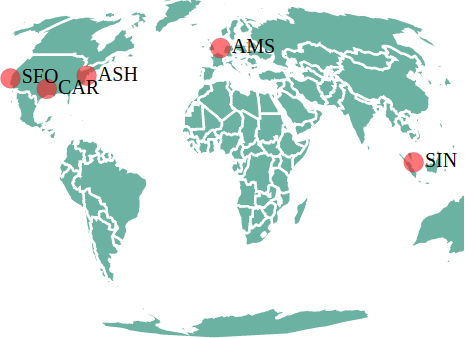
\includegraphics[scale=0.45]{building_energy_model/img/dc_locations.png}
\caption[DC Locations]{Data Center Locations Map. SFO: San Francisco, CAR: Carrolton, TX, ASH: Ashburn VA, AMS: Haarlem, Netherlands, SIN: Singpore.}
\label{fig:dc_map}
\end{figure}

One issue with the Kaggle data set is that it just provides a time series of page visits agnostic of source location (ie user location) or serving DC. For evaluating DC level workloads, the pages were mapped to a DC \added{location} as part of a pre-processing step of this research. The pre-processing required \added{handling} raw URL strings and parsing out it's language hash markers. Then, countries where these languages are the official languages are mapped to the nearest Wikipedia DC to indicate the traffic to each DC. \added{The step-wise procedure is in indicated in Table~\ref{table: url2dc}.}

\begin{table}[!h]
\caption[Steps to convert Raw URL to DC Network Traffic]{Steps for converting URL to traffic} \label{table: url2dc}
\begin{small}
\begin{tabular}{c|l}
\hline \hline
Step 1:& Map language to page by parsing URL \\
&structure. \\
\hline
Step 2:& Map languages to countries where they \\
& are the first tongue. \\ 
\hline
Step 3:& Map ingress sites to countries with \\
& minimum distance function. \\
\hline
Step 4:& Get the distribution of the number of \\
& countries served by each ingress site. \\
\hline
Step 5:& For each ingress site; sum up the daily \\
& views of pages in all language. \\
\hline \hline
\end{tabular}
\end{small}
\end{table}

The procedure resulted in the seven languages being routed by a minimum distance function from any country that they are the official language to the nearest DC site. Treating each of the seven languages as a service \deleted{allows this research to have an abstraction of the (Moriyama , et al., 2018) service which is intuitive to reason about as indicated in Figure~\ref{fig:lang2dc}} \added{provides an abstraction that makes each language an isolated platform. 

Figure~\ref{fig:lang2dc} shows curves with all languages to a particular data center aggregated together. These curves are translated to a coefficient that scales the IT load indicated on line 8 of Figure~\ref{ite_object}. The coefficients for each data center are normalized to the maximum traffic volume; i.e. max traffic indicates the upper bound with a coefficient of 1. These coefficients are independent across the five data centers.}

\begin{figure}.
\centering
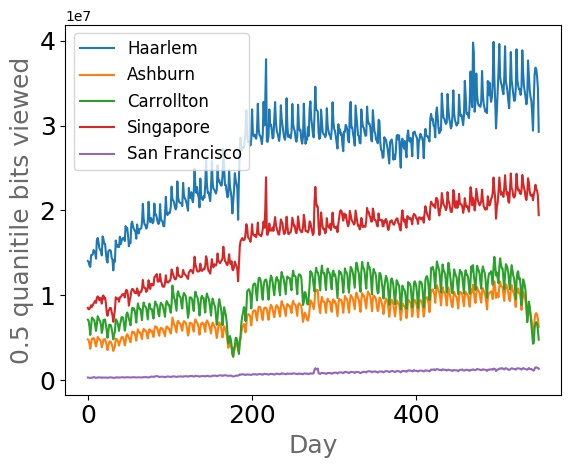
\includegraphics[scale=0.45]{building_energy_model/img/lang2dc_curve.jpg}
\caption[DC traffic with all languages summed]{Sum of English, French, German, Mandarin, Spanish, Russian, and Japanese traffic to each of the 5 DC locations.}
\label{fig:lang2dc}
\end{figure}

\deleted{To validate the impacts of resetting the proportional load factors, two specific simulations were run for each of the DCs from Figure~\ref{fig:lang2dc} The first is the novel dynamic load simulation and second configured as in \citep{moriyama18}. In both simulations nominal power density of the DC is set to 2kW/m2 and the auto-sizing feature is enabled for all HVAC equipment.} 


\deleted{\textit{Algorithm} \ref{Service Profile} indicates how the the service demand profile is generated. It is based on Kaggle's web-traffic data-set $(K)$ which is a time-series of the count of visits $(v)$ to 145,063 Wikipedia pages distributed across seven languages $(l)$ at daily intervals \citep{kaggle17}. In this work  pages $(p)$ are aggregated together by language and classified as a common service. $P_l$ is a list of all pages with the language $l$. The subscript $d$ represents individual DCs.  The demand for the service at a particular DC is obtained by the average quantile visits to the pages of the respective language as indicated by $P_{l}[d]$.} 

\deleted{\begin{algorithm}
\caption{Service Profile}
\begin{algorithmic}[1]
\REQUIRE{$K$} %Time series
	\FOR{$p$ in $K$} % Each Page in the time T
		 %For each lanugauge in T
		\STATE{$P_l = empty[$ $]$} % Create a unique table for each lanuage
		\STATE {$P_{l}[l] \gets p_l == l$  } % Populate matching langauge intot he luange table
		\FOR{$d$ in $range(K_d)$}
			\STATE {$P_{l}[d][quantile(v)] \gets \sum{P_{l}[l][d]}$} %Sum the visits, v per day to get service profile
	\ENDFOR
	\ENDFOR
\end{algorithmic}
\label{Service Profile}
\end{algorithm}}

\deleted{Figure~\ref{fig:lang2dc} illustrates the service profile for the data range and notes the seven languages. The y-axis is the number of page views on a $1e^8$ scale, the x-axis spans the date range, and the curves represent each of the seven languages.}
Next we discuss the results from a model build with the methods discussed in this section.

% -------------------------------------------------------------------------------------------------------------------------------
\section{Results}
% -------------------------------------------------------------------------------------------------------------------------------

\added{The traffic aware EnergyPlus models are simulated for each data center location through GymEplus in a batch process loop. In the batch workflow, the same IDF file is used to represent all of the data centers shown on the map in Figure~\ref{fig:dc_map}, except their local weather files are changed by the scripted loop. In} these reset load (RL) simulations, \added{at each time step} the traffic load factor is pulled in \deleted{by}\added{from} the Python program and is passed to EnergyPlus \added{by BCTVB. This demonstrates that using an external interface (such as logic scripted in Python), building energy models can facilitate the analysis of a network of data centers in a single workflow. 

A second set of simulations without the external interface (NoRL) were also run for each DC with a similar workflow to quantify the energy use with default CPU loading schedule shown in Figure~\ref{cpu_load_reset}.} The total annualized energy use of the two models is plotted for comparison in Figure~\ref{fig:total_energy_comp_bem}. The purple bars indicate the simulations in which the CPU loads are reset at each time-step (RL), and the green bars indicate simulations without interactive resetting of the loads (NoRL). For Singapore (sin), San Francisco (sfo), and Ashburn (ash) the RL simulations result in higher annualized energy compared to the NoRL model. While for Amsterdam (ams) and Carrolton, TX (car), the RL model results in lower energy demand compared to the statically configured load from the NoRL simulation.

\begin{figure}.
  \centering
  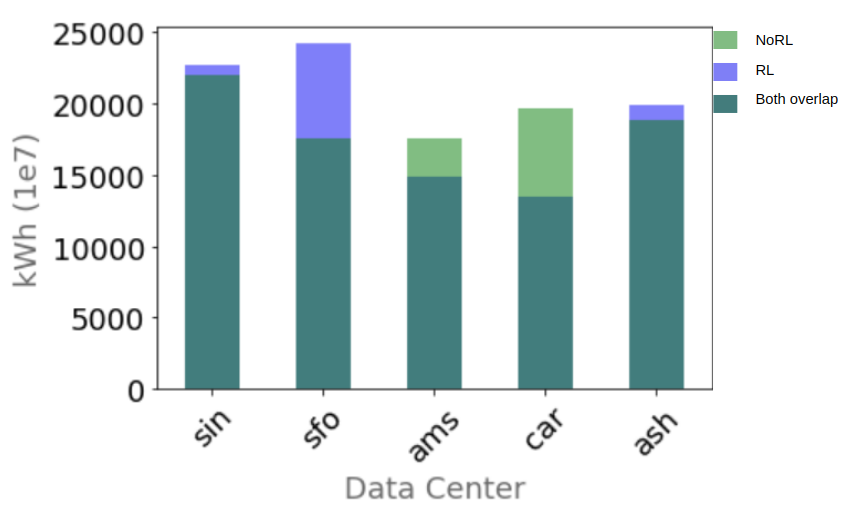
\includegraphics[scale=0.4]{building_energy_model/img/cpu_comps_3legend.png}
  \caption[Comparison of energy demand for two models]{Total Site Energy Difference between statically configured IT load and dynamically reset IT loads.}
  \label{fig:total_energy_comp_bem}
  \end{figure}

The variations in the relative energy demands between the two models can be attributed to the CPU load profiles as illustrated in Figure~\ref{fig:cpu_comps}. The figure illustrates the time series plot of each DC analyzed through the RL simulations with line curves. The x-axis indicates the hour of the year and the y-axis indicates the CPU load for each respective DC. \deleted{Examining}\added{The CPU profiles for each DC that} their \deleted{values appear quite}\added{average values} are distinct from one another. Carrolton and Ashburn appear to have  \deleted{strong}\added{noticeable} seasonal patterns. Amsterdam and Singapore DCs show irregular oscillations in demand throughout the year\added{, but have a tight band}. The San Francisco DC has a constant line. This constant demand is due to the load not varying much from the peak capacity in the traffic profile that was used for the site. 

In contrast to the distinct CPU load profiles of the RL loads as discussed above, with default schedule configuration of IT load profiles used in the NoRL models, the CPU loads at all the DCs are identical to each other. The static property of the NoRL model is also indicated in Figure~\ref{fig:cpu_comps} by the gray band. The gray band is actually composed of line curves that cycle diurnally with the given schedule.


\begin{figure}
  \centering
  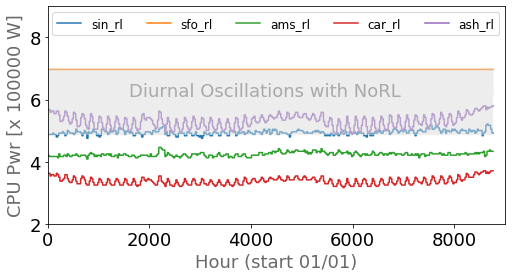
\includegraphics[scale=0.45]{building_energy_model/img/cpu_comps.png}
  \caption[CPU Time Series]{Time series of the total CPU power at each DC (see legend). Gray area indicates the daily demand cycle that the IT equipment creates with NoRL.}
  \label{fig:cpu_comps}
  \end{figure}

\deleted{Given this understanding of the cyclic loads, the relative variance between the RL and NoRL simulation’s total energy results can be reasoned about by considering the profile of San Francisco DC as an extreme example. San Francisco’s RL model does not vary the CPU load, whereas the NoRL model does. With the constant peak load, the San Francisco DC’s RL simulation indicates higher utilization than the NoRL model therefore demanding more power.}

\added{Figure~\ref{fig:stacked_pue} shows a stacked histogram for the set of DCs modeled. This plot shows that even with a identical building systems the efficiency of each DC will vary across the globe. One major contributor to this difference is obviously the local weather conditions which DC operators can;t control. However, the second contributor is the workloads at the DC. The workload is a variable that can be controlled by the DC operators.}

\begin{figure}[!h]
  \centering
  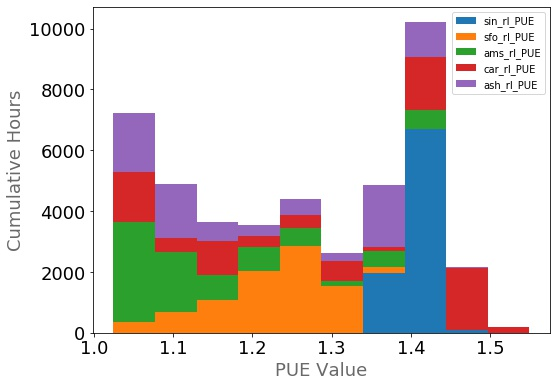
\includegraphics[scale=0.4]{building_energy_model/img/pue.jpg}
  \caption[Stacked PUE Histogram]{Stacked PUE Histogram for all five data centers .}
  \label{fig:stacked_pue}
  \end{figure}

In the next section, the extensibility of the traffic based building energy model towards predicative scenarios and the potential to use this framework to exploit 'free capacity' are discussed.  


%-------------------------------------------------------------------------------------------------------------------------------
\section{Discussion}
% -------------------------------------------------------------------------------------------------------------------------------
\deleted{To reason about the EnergyPlus RL results from Figure~\ref{fig:total_energy_comp} for total energy, the San Francisco site again serves as an example. In the figure, the total site energy used for the annual model is $1.19 \times 10^7$kWh. Through the course of 8,760 hours the power demand for the DC is 1,359 kWh on average; translating to an annualized PUE value of approximately 1.36 due to the base IT load density of $2 kW/m^2$ (with a network load coefficient set to 1 for all hours). The PUE values of the other sites are more complex to reason about without further processing of the data, as they all operate at part load conditions.}

One obstacle for building operators for using building energy models to make operational decisions is that working with these models requires deep knowledge about the software implementation of the models. The one variable that operators control are the IT loads and allowing the IT loads to characterized by external software in building energy models can allow operators to do some interesting things. For example, operations teams can simulate perceived future changes to their work loads. As mentioned above predicative modeling is feasible when using network traffic as the proxy for IT loads. Network traffic has been shown to be predictable within reasonable accuracy for internet services by Linkedin \citepp{zhuang15}. Figure~\ref{fig:arima_bem} shows the predicative models for four of the data center studied in the simulations for this work. 


\begin{figure}[!h]
  \centering
  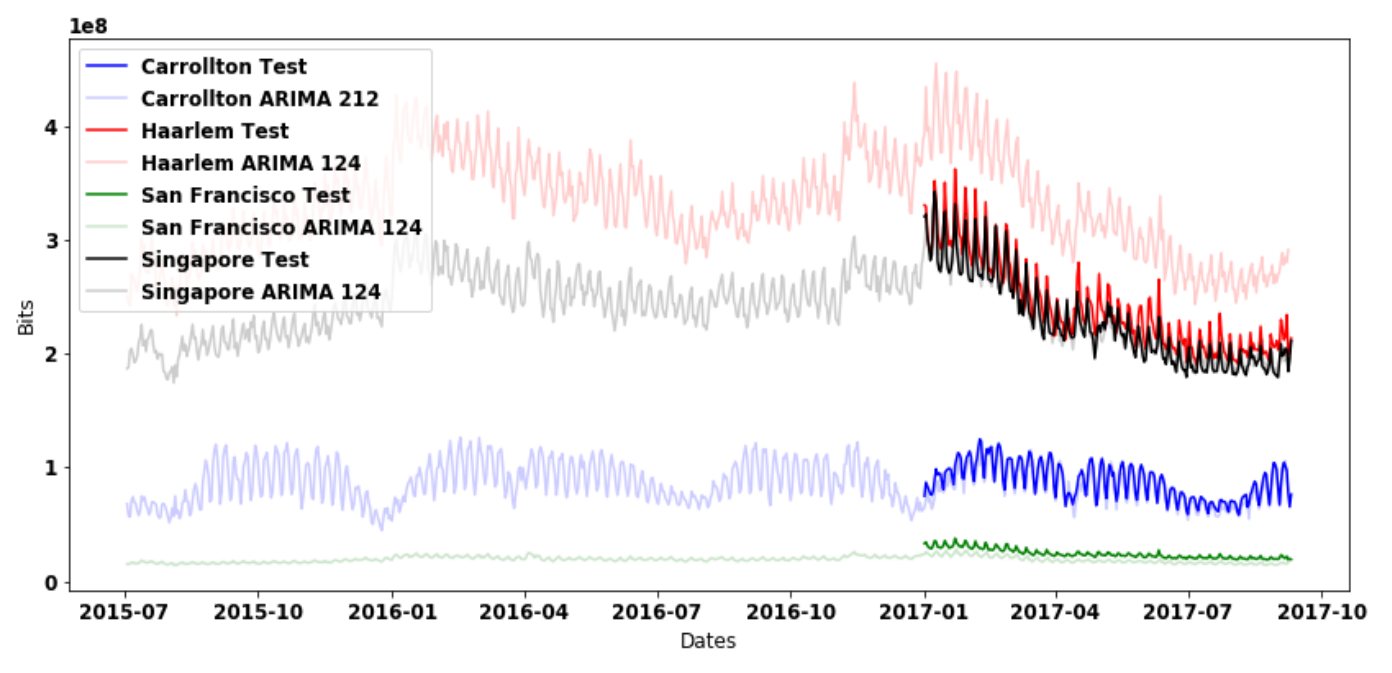
\includegraphics[scale=0.25]{img/_arima.png}
  \caption[ARIMA for BEM]{Forecasting Model of the Traffic.}
  \label{fig:arima_bem}
  \end{figure}

In this research the network traffic serves as a proxy for CPU utilization. In practice the network traffic and CPU have complex correlations that can't be generalized with the presented approach. In production DC environments representative correlations can be obtained between network traffic, the IT workloads the the traffic instantiate, and the workload's CPU demand. However, proving such correlations is out of scope of research. \added{Nonetheless, every data center will be subject to its own traffic models due to it being an intrinsic property of the service.}

This research assumes that all the facilities are of the same size in terms of power, space, and cooling. From looking at Figure~\ref{fig:lang2dc}, San Francisco site has a much lower traffic profile than Haarlem. The claim that the same power capacity handles this range of traffic requires another assumption. This assumption is that the CPU-Network ratio vary from site to site. For example a bit of network traffic generates 40 times as much CPU workload in San Francisco as it does in Haarlem. This assumption is the basis for normalizing the traffic coefficient, as described by the discussions on Figure~\ref{fig:lang2dc}. This is a realistic condition in DC fleets were have different generations of IT hardware in operations at various DCs. Or this condition can be encountered when software optimizations to specific workloads are done for targeted consumer markets that are geographically segregated. Nonetheless, since the network coefficient is bound between 0 and 1, and network-workload-CPU model can be supported in the same framework. 

\added{As an example of free capacity mentioned above, consider a design day dry-bulb temperature of 105$^{\circ}$F. When a peak in IT workload occurs on a more favorable day, say 95$^{\circ}$F, the computer room air conditioner heat rejection equipment needs 50\% of the designed power value \citep{liebert20}. With a slight modification in the electrical infrastructure, this difference can opportunistically be allocated to IT workloads. However, slight the the electrical modification, the decision is most cost effectively made during the design phase of the the facility. This influence on the design presents a case for using the fine grained load aware model presented incpu\_load\_reset the work during the design phase as-well.

Opportunistically using 50\% of the provisioned power from the cooling equipment to power the IT equipment requires some further insights about DC operation. First, the 50\% claim is based on nameplate full load amps (FLA) for two different dry-coolers (Models D-466 & D-880) are matched with a 105kW indoor computer room air conditioner (DC Model 105). One of the dry-coolers is rated at 95$^{\circ}$F and the other is rated at 105$^{\circ}$F \citep{liebert20}. The FLA for these units are 14 Amps and 28 Amps respectively. Physically this translates to breaker sizes, wires sizes, utility power feed reservations, and back-up generator reservations decisions being made using this value. Second, with the claim it is assumed that the power draw has the same proportional scaling with loads cross both sets of units. 

To summarize the last two paragraphs more explicitly, in conditions where the ambient enthalpy is lower then the design day, \deleted{the additional capacity of the cooling equipment are}\added{electrical provisions beyond the real-time demand relative to the design values are} stranded. \added{This is an important consideration for a building class where its utility is measured by the power delivered to IT equipment use. Anytime when the stranded power can be re-purposed from auxiliary infrastructure (such as chillers, cooling towers, and transformers) to the IT equipment, it leads to compelling return on investment cases.}

% This is a naive assumption and such a practice is not suitable for the design phase building energy models where equipment must be sized for worst case conditions. However, the claim suffices to demonstrate that on non design days there is stranded power in terms of the physical capabilities of the electrical infrastructure. For a building class where its utility is measured by IT power density; any opportunistic usage of power is highly valuable. As a concrete example, when the part load of the dry cooler is known for future states in time, major capacity constraints in DC such as the utility power reservations and back up generator reservations can be relaxed during that time range. This would allow the IT to be oversubscribed relative to its design conditions, yet the building would still be within its overall power envelope. 

%\added{utility power reservations and back-up power generator reservations. More explicitly, during the part load operations of the cooling plant when their electrical demand is lower then their design values; the headroom in power infrastructure from the cooling equipment can be safely supplied to IT equipment. The rerouting of the available power increases the supportable IT load and essentially yields 'free capacity' beyond the design values of the IT load}% 
}

% \added{The design power input represents the electrical power loading of servers. In practice the CPU is a dominate energy consumer of IT equipment but it’s not the only power consumer. Aside from the fan and power supply unit which are explicitly defined in the ITE IDF object, it is unclear how the power demand for hard disks, random access memory, and other parts are accounted for in EnergyPlus.}

% Another benefit for externally configuring traffic changes to the data centers is that when new data centers are built, the traffic routing changes. Having an external signal for the traffic allows operators to run the models to check operations without having to change the building systems.

%Independently normalizing each data center to max workload is sensible as each data center may have different hardware with various performance behaviors. For example it may take more resource at one site to complete a user request as it does at another site.
% -------------------------------------------------------------------------------------------------------------------------------
\section{Conclusion}
% -------------------------------------------------------------------------------------------------------------------------------
There are two notable benefits of resetting the IT load values outside of the IDF file. First, defining load values for each hour in the IDF file is toilsome and error prone. The toil of entering values for each simulation time-step would require 8,760 entries in the file. This increases the chance of introducing errors into the simulation. Second, the external definition allows more sophisticated logic to control the time-step variables. In this article, only the IT load factors were reset, none-the-less the same interface can reset many other simulation run-parameters with similar logic. An example of a feedback logic is reinforcement learning, which can be framed to globally optimize the systems and is an topic for future research. 

The traffic profile used in this article are representative of a globally distributed service’s user facing workloads and suffices for purposes of demonstrating the dynamics of DC operational loads. Each real-world service will have a unique profile resulting from a combination of critical and opportunistic back-end workloads. The modular construction of this model is conducive for incorporating the other workloads and being inclusive of back-end workloads.

Figure~\ref{fig:lang2dc} aggregates all the languages to provide an overall building simulation. However future work that need to assess a service platform can create multiple ITE objects in EnergyPlus and quantify the energy demands for each in isolation.